\section{Grundlagen}
\label{sec:grundlagen}

In diesem Kapitel gilt es zu klären, auf welchen Grundlagen, Ideen und Konzepten Model-View-Intent beruht, wie diese miteinander fungieren und weshalb sie als Inspiration dienten.

\subsection{Unidirektionaler Datenfluss und der Zustand: Flux, Redux und Elm}

In einer Applikation existieren grundsätzlich zwei Komponenten: Eine, die der Nutzer wahrnehmen kann und eine, die für ihn unsichtbar bleibt. Bei ersterer handelt es sich meist um das, was der Nutzer(auf dem Bildschirm) sieht - die sogenannte »View«. Die zweite Komponente beschreibt die Ebene, welche das Geschehen observiert, darauf reagiert und den weiteren Verlauft (zum größten Teil) kontrolliert. Sie kann unter anderem als »Controller« betitelt werden.
\\
\\
Ein weiterer, essentieller Aspekt einer Anwendung ist ihr Zustand. Dieser kann sich aus mehreren Teilen zusammensetzten:
\begin{itemize}
	\item Alles was der Nutzer sieht
	\item Daten die über das Netzwerk geladen werden
	\item Standort des Nutzer
	\item Fehler die auftreten
	\item \dots
\end{itemize}
Der Zustand in dem sich eine Applikation befindet kann hierbei von beiden Seiten modifiziert und beobachtet werden. Ist dies der Fall, so handelt es sich um einen bidirektionalen Datenfluss. Bei dieser Variante entsteht die eventuelle Gefahr von kaskadierenden Updates (ein Objekt verändert ein anderes, welches wiederum eine Veränderung bei einem weiteren herbeiführt usw.) als auch in einen unvorhersehbaren Datenfluss zu geraten: Es wird schwer, den Fluss der Daten nachzuvollziehen. Des weiteren muss immer überprüft und sichergestellt werden, dass »View« und »Controller« synchronisiert sind, da beide den globalen Zustand darstellen. Schlussendlich verliert man zusätzlich die Fähigkeit zu entscheiden, wann und and welcher Stelle der Zustand manipuliert wird.
\\
\\
Ein anderer Ansatz ist, den Datenfluss in eine Richtung zu beschränken und ihn damit unidirektional
\cite{unidirectionalDataFlowFluxArchitectureIlyGelman2017, unidirectionalDataFlowTheCompleteReduxBookIlyGelman2017}
operieren zu lassen. Diese Variante erfreut sich an zunehmender Popularität seit der Bekanntmachung der »Flux«
\cite{fluxArchitectureAdamBoduch}
Architektur im Jahre 2015 von Facebook.
\cite{fluxAnnouncementYoutube}

\subsubsection{Flux}
Für die Einhaltung und Umsetzung eines unidirektionalen Datenfluss und der Verwaltung des Zustands bedient sich »Flux« bei zwei fundamentalen Konzepten: Der Zustand innerhalb einer Applikation wird als »single source of truth (SSOT)« angesehen und darf keine direkte Änderung erfahren. Um dies zu Gewährleisten finden sich mehrere Komponenten in »Flux« wieder:
\\
\\
\textbf{Action}: Eine Aktion beschreibt ein Ereignis, welches unter anderem vom Nutzer ausgelöst werden kann. Sie geben vor, wie mit der Anwendung interagiert wird. Jeder dieser Aktionen wird dabei ein Typ zugewiesen. Insgesamt sollte eine Aktion semantisch und deskriptiv bezüglich der Intention sein. Des weiteren können zusätzliche Attribute an eine Aktion gebunden werden.
\\
\begin{lstlisting}[frame=single, language=Java]
{
 type: ActionTypes.INCREMENT,
 by: 2
}
\end{lstlisting}
\bigskip
\textbf{Dispatcher}: Er ist für die Entgegennahme und Verteilung einer Aktion an sogenannte »Stores« zuständig. Diese haben die Möglichkeit sich beim ihm zu registrieren. Er besitzt die wichtige Eigenschaft der sequentiellen Verarbeitung, d.h., dass er zu jedem Zeitpunkt nur eine »Action« weiterreicht. Sämtliche »Stores« werden über alle Aktionen unterrichtet.
\\
\\
\textbf{Store}: Hier befinden sich die Daten, welche einen Teil des globalen Zustands einer Anwendung ausmachen. Die einzige Möglichkeit für eine Veränderung der dort hinterlegten Daten besteht durch ein Reaktion auf eine, vom »Dispatcher« kommenden, Aktion. Bei jeder Modifikation der Daten erfolgt die Aussendung eines Events an eine »View«, das die Veränderung mitteilt.
Ebenso findet sich hier ein Part der Anwendungslogik.
\\
\\
\textbf{View}: Die View ist für die Anzeige und Eingabe von Daten zuständig - sie ist die für den Nutzer sichtbare Komponente, mit welcher dieser interagiert. Ihre Daten erhält sie von einem »Store«, diesen sie abonniert und auf Änderungsereignisse hört. Erhält sie vom »Store« ein solches Änderungsereignis, so kann sie die neuen Daten abrufen und sich selbst aktualisieren. Der View ist es nicht gestattet, den Zustand direkt zu verändern. Stattdessen generiert sie eine Aktion schickt diese an den Dispatcher.
\\
Ein Beispielhafter Ablauf bei einer Anwendung die einen Wert erhöht oder verringert kann wie folgt aussehen:
\begin{enumerate}
	\item Die View bekommt einem Store zugewiesen, welcher für das inkre- und dekrementieren der angezeigten Zahl verantwortlich ist.
	\item Sie erhält die Anfangszahl und stellt diese in einem leserlichen Format/einer Ansicht dar, welches es dem Nutzer ermöglicht, damit zu interagieren.
	\item Betätigt dieser einer der Knöpfe welche die dargestellte Zahl verändern, so wird eine Action erstellt und an Dispatcher geschickt.
	\item Dieser wiederum informiert alle Stores.Information
	\item Jener Store der für die Verarbeitung dieser Aktion verantwortlich ist, modifiziert die Zahl in seiner internen Datenstruktur und kommuniziert dies über ein Änderungsereignis
	\item Diejenige View, welche auf Änderungsereignisse diesen Ursprungs lauscht, erhält die Daten und aktualisiert sich dementsprechend. 
\end{enumerate}

\begin{figure}[ht]
	\centering
	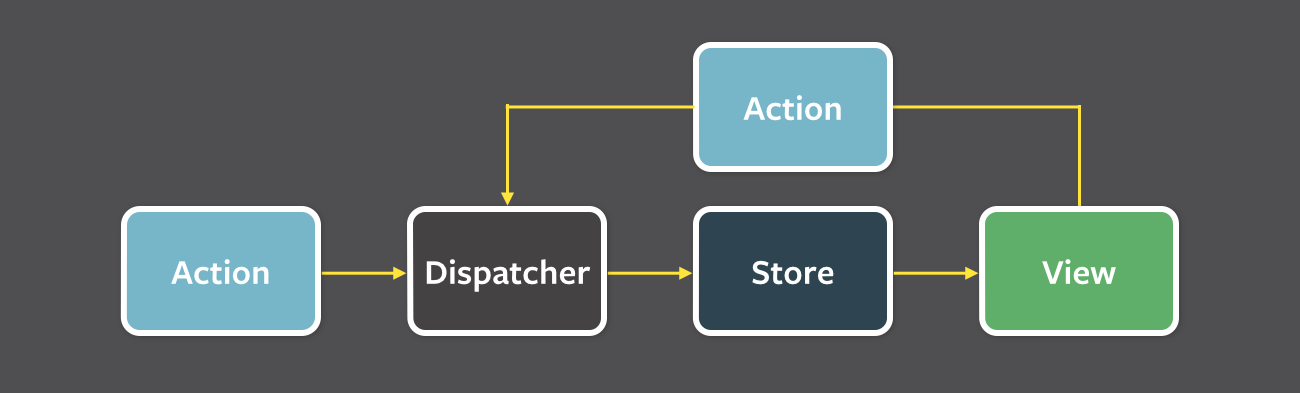
\includegraphics[height=0.25\textwidth]{./images/flux-flow}
	\caption{Datenfluss in der Flux Architektur}
	\label{fig:datenflussFlux}
\end{figure}

Anhand Abbildung \ref{fig:datenflussFlux} wird der unidirektionale Datenfluss deutlich erkennbar:
\begin{enumerate}
	\item Die View schickt eine Aktion an den Dispatcher.
	\item Dieser leitet diese an alle Stores weiter.
	\item Der Store verarbeitet die Daten und informiert die View.
\end{enumerate}
\bigskip
Insgesamt liefert Flux mit diesen Komponenten eine Möglichkeit, einen unidirektionalen Fluss herzustellen und die Verwaltung des Zustands einer Applikation zu vereinfachen.
\subsubsection{Redux}
\label{subsec:redux}
Bei Redux handelt sich um eine JavaScript Bibliothek (und kein Framework) welche ihre Inspiration aus Flux und Elm bezieht. Sie wurde im Jahre 2015 von Dan Abramov und Andrew Clark ins Leben gerufen.
\cite{reduxIntroduction}
Auch hier nimm der direktionale Datenfluss eine wesentliche Rolle ein.
\\
\\
Die Bibliothek kann als eine vereinfachte Form von Flux verstanden werden, welche gewisse Elemente und Ansätze übernimmt, aber auch streicht bzw. ersetzt. Genau wie Flux existieren die bereits behandelten Actions, welche über wichtige Informationen für die spätere Veränderung des Zustands verfügen. Auch hier können diese ihren Ursprung in einer vom Nutzer getätigten Aktion haben. Wird eine Aktion ausgeführt, so spricht man von einer Versendung einer Aktion. Dieser Versand findet nur dann statt, wenn man die Intention verfolgt, den Zustand zu ändern. Sie gelangt zu einem sogenannten "Reducer". Hier findet sich der erste Grundlegende Unterschied zu Flux.
\\
\\
Ein "Reducer" ist für sich genommen eine einfache Funktion, die bei gleicher Eingabe die immer gleiche Ausgabe erzeugt. Sie ist dabei frei von sogenannten Seiteneffekten und wird als "pure" bezeichnet. Im Falle eines "Reducers" erwartet dieser die vorher erzeugte Aktion und den globalen, derzeitigen Zustand der Anwendung. Sein Aufgabe ist es, aus der Kombination dieser einen neuen Zustand zu generieren. Hierfür wird die Aktion, basierend auf ihrem Typ und eventuellen Inhalt, ausgewertet und der Zustand dementsprechend angepasst. Dabei ist zu beachten, dass keine direkte Manipulation des Zustands möglich ist, stattdessen wird ein komplett neuer Zustand zurückgegeben. Diese Eigenschaft der Unveränderbarkeit wird gemeinhin als "Immutability" erfasst.
\\
\begin{lstlisting}[frame=single, language=Java]
(previousState, action) => newState
\end{lstlisting}
\ \\
Das Verbindungsstück zwischen einer Aktion und dem Reducer bildet der Store. Dieser existiert im Gegensatz zu Flux nur ein einziges Mal (und mit auch der Zustand) und ist für die Verwaltung des Zustands verantwortlich. Er übernimmt zugleich auch die Rolle des Dispatchers, wie er in Flux vorkommt, und verteilt die Akionen an alle Reducer weiter. Der aus dem diesen Prozess hervorgehende, neue Zustand wird im Store hinterlegt. Dieses Ereignis wird ebenfalls seitens der View observiert, welche im Anschluss die nötigen Aktualisierungen an der Ansicht vornimmt.
Am Ende lässt sich der gesamte Fluss wie folgt darstellen:
\\
\begin{lstlisting}[frame=single, language=Java]
View -> Action -> Reducer(s) -> Store -> View
\end{lstlisting}
\bigskip
Neben Redux existieren in der JavaScript Welt noch weitere Bibliotheken, die entweder eine Abwandlungen von Flux darstellen oder aber neue Konzepte implementieren. Jedoch verfolgen dabei alle eine ähnliches Ziel: Ein unidirektionaler Datenfluss und die (zentrierte) Verwaltung des Zustands einer Anwendung.

\subsubsection{Elm}
Bei Flux und Redux handelt es sich jeweils um Bibliotheken die innerhalb einer Anwendung verwendet werden können. Eine weitere Herangehensweise ist die Verankerung solcher Konzepte in der Programmiersprache selbst. Dies findet man z.B. in
der Programmiersprache Elm
\cite{elmIntroduction}
wieder. Elm besitze eine in die Sprache integrierte Architektur die den einfach Namen "The Elm Architecture" 
\cite{theElmArchitecture}
trägt. Eine andere Variante lautet: Model-View-Update. Anhand dessen lassen sich bereits die Kern-Komponenten der Entwurfsmusters erahnen.
\\\\
\textbf{Model:} Dies repräsentiert den Zustand der Applikation als eine simple Datenstruktur.
\\
\textbf{View:} Sie ist eine Funktion, welche aus einem Model HTML code generiert. Ebenfalls wie in Flux wird kommt auch hier das Konzept von "pure functions" zum tragen: Die gleiche Eingabe erzeugt die gleich Ausgabe - ohne Ausnahme.
\\\\
\textbf{Update:}
Hierbei wird, ähnlich wie im 'Reducer', das Model manipuliert und dadurch der Zustand der Anwendung aktualisiert.
\\\\
Es ist zu erkennen, dass diese Architektur den vorherigen sehr ähnlich ist. Sie genießt jedoch den Vorteil ein wesentlicher Bestandteil der Sprache zu sein. Damit ist es unter anderem möglich, die Sprache auf die Architektur anzupassen, statt andersherum.

\subsection{Funktionale Programmierung}
Im Verlaufe der Kapitel wurden bereits Begriffe wie eine "reine" Funktion ('pure functions') oder die Unveränderlichkeit einen Datenstruktur angesprochen. Diese Konzepte zählen zu einem Programmierparadigma, welches in den letzten Jahren auch an Bedeutung in Sprachen wie Java gewonnen hat
\cite{javaFunctionalProgramming}
: funktionale Programmierung.
\\\\
In der häufig imperativen, objektorientierten Programmierung wie sie in Java oder auch C\# anzutreffen ist, machen Klassen, die Mutation derer und globale Variablen den Hauptbestandteil des Quellcodes aus. Dabei ist zu beachten, dass die funktionale Programmierung die Objektorientierte nicht zwingenden ausschließt, sondern lediglich in eingeschränkter Form nutzt. In der funktionalen Programmierung geht es, wie der Name bereits vermuten lässt, hauptsächliche um das Arbeiten mit Funktionen.
\\\\ 
Dabei muss man verstehen, das bei einer imperativen Entwicklung Schritt für Schritt programmiert wird, wie etwas getan werden soll. Es handelt sich dabei oft um eine Serie von Mutationen in Kombination mit Abfragen von gewissen Konditionen. In der funktionellen hingegen wird nur zum Ausdruck gebracht, das etwas vollführt werden soll, aber nicht wie es am Ende vollbracht wird. 
\\\\
'Funktionale' Funktionen sind nicht identisch mit den 'unreinen' Funktionen, die beispiel- oder typischerweise in Java genutzt werden - die, die einen Wert zurückgibt (oder nicht). Stattdessen ist eine funktionale Programmierfunktion wie eine mathematische Funktion, die eine Ausgabe erzeugt, die ausschließlich von ihren Argumenten abhängig ist. Jedes Mal, wenn diese mit den gleichen Argumenten aufgerufen wird, erhält man immer das gleiche Ergebnis. Erreicht wir dies durch Funktionen, die Frei von Seiteneffekten sind. Das bedeutet, dass keine globale Variable mutiert oder bspw. auf die Konsole ausgegeben wird. Ebenfalls sind Operation die auf die Peripherie des Gerätes zugreifen (I/O) theoretisch nicht erlaubt. Somit ist ein  Seiteneffekt ein extern beobachtbarer Effekt, den eine Funktion zusätzlich zur Rückgabe eines Wertes ausführt. Im Prinzip sorgen sie für inkonsistente Abläufe bzw. Resultate innerhalb eines Programms. Natürlich ist die Entwicklung einer Anwendung ohne Seiteneffekte unmöglich, daher geht es vielmehr darum, sie zu minimieren und gesondert zu behandeln. Sie sollten meist am Ende einer Berechnung erfolgen und nicht im Laufe dieser.
\\\\
Für die Einhaltung dieser Prinzipien stellt eine funktionale Sprache meist unterschiedliche Werkzeuge zur Verfügung. Dazu gehören Funktionen höherer Ordnung, bei der eine Variable eine Funktionen verkörpern kann. Die tief verankerte Fähigkeit unveränderliche Datenstrukturen zu erstellen. Das arbeiten mit Klassenhierarchien und algebraischen Datentypen, sowie dem oft dazugehörigen Musterabgleich. Oder die Bereitstellung von sogenannten 'Monads', welche unter anderem dafür dienen Seiteneffekte zu isolieren und erkennbar zu machen.
\\\\
Ein großer Vorteil der funktionalen Programmierung ist, das vieles ein deterministisches Verhalten aufweist. Dies macht es einfacher einen Überblick zu bekommen und das Programm zu verstehen. Zugleich macht die Komposition von Funktionen das Programm modularer. Ein weiterer nicht zu unterschätzender Vorteil entspringt der Unveränderlichkeit, durch welches die Anwendung Threadsicherheit erlangt.
\\\\
Insgesamt kann gesagt werden, dass das Anwenden von funktionalen Konzepten auch in Sprachen wie Java angestrebt werden sollte. Selbst wenn dies nicht in dem Umfang stattfinden kann, wie es in 'echten' funktionalen Sprachen möglich ist. 
\\
Zuletzt sollte noch erwähnt werden, dass am Ende immer imperativer Code steht. Funktionale Programmierung stellt eine Abstraktion dar und ist intern imperativ.

\subsection{Reaktive Programmierung}
\label{subsec:reaktive-programmierung}
Heutige Anwendungen müssen viele Ereignisse in scheinbar willkürlicher Reihenfolge verarbeiten: Ein Klick eines Nutzer, eine Fehlermeldung, Speichern im Dateisystem, Kommunikation mit dem Netzwerk, aktualisieren der Benutzeroberfläche usw. Auf jedes dieser Ereignisse muss das Programm reagieren, und dabei immer Ansprechbar bleiben. Hierfür ist es Notwendig den Code asynchron zu schreiben, d.h. ohne das andere Prozeduren blockiert werden.
\\\\
Ein bekannte Methode stellt hierbei die Verwendungen von sogenannten Rückruffunktion ('Callbacks') dar, welches ein gern genutztes Mittel in der imperativen Welt ist. Leider führt diese Variante meist zu einer 'Callback Hell' und tief verschachtelten, unübersichtlichen Code. Dazu existieren vielfältige Verbesserungen, die alle eins Gemeinsam haben: sie reagieren (auf etwas).
\\\\
Hierzu besteht ein weiteres Paradigma: die reaktive Programmierung. Sie setzt auf Konzepte der funktionalen Programmierung, bevorzugt einen deklarativen Ansatz und ist damit eine weitere Abstraktion. Ihr anliegen ist es, asynchronen Code basierend auf unterschiedlichen, zeitlich abhängigen Ereignissen einfach zu handhaben.
\\
Ein Beispiel ist das Tippen auf einen Touchscreen; etwas, dass zu beliebigen Zeitpunkten passieren kann. Anstatt in einer Schleife zu fragen 'Hat der Nutzer den Bildschirm berührt?' hinterlegt man beim System etwas das auf dieses Ereignis horcht. Registriert das System eine solche Aktion leitet es dies Information an alle 'Zuhörer' weiter. Über diese Vorgehensweise können die unterschiedlichsten Datenquellen angesprochen werden. In der reaktiven Programmierung ist es möglich mehrere solcher Ereignisse zu Kombinieren und mit ihnen zu arbeiten.
\\\\
Zum Einsatz kommt in der reaktiven Programmierung das Beobachter-Muster (Englisch Observer Pattern). In diesem wird eine Änderung an einem Objekt an alle die von ihm Abhängig sind propagiert. Dabei unterscheidet man zwischen einem 'Observable' und dem 'Observer'. Ersterer erzeugt ein oder mehrere Ereignisse und bietet Operatoren um mit ihnen zu arbeiten. Daraus ergibt sich ein Fluss an Daten, der von jemanden aufgenommen und beobachtet werden möchte - dafür ist der 'Observer' zuständig. Dieser schließt eine Abonnement auf dem 'Observable' ab und erhält die gewünschten Daten. In Pseudocode kann dies wie folgt aussehen:
\begin{lstlisting}[caption={Pseudocode reaktive Programmierung}, label={lst:pseudo-reaktiv}, language=Kotlin]
Observable.produce("Hello")
	.delay(1000)
	.map { text -> text + " World" }
	.subscribe(SomeObserver())
\end{lstlisting}
\bigskip
Am Beginn von Listing 
\ref{lst:pseudo-reaktiv}
wird eine Wert erzeugt, als 'Observable' transferiert und um 1 Sekunde verzögert. Genau wie bei der funktionalen Programmierung ist dabei die Implementation von 'delay' zweitrangig. Es geht nur darum auszudrücken was gemacht werden soll und nicht wie. Dies hat zur Folge, dass der Code ausdrucksstark wird. Als nächstes wird mit einer anonymen Funktionen höherer Ordnung der Wert manipuliert. Zum Schluss hinterlegt sich der 'Observer' als Abonnent und erwartet das Resultat. Abgesehen von der 'subscribe' Funktion gibt jede andere ein neues 'Observable' zurück. Das liegt daran, dass das 'Observable' als unveränderliche Datenstruktur realisiert wird.
\\\\
Reaktive Programmierung macht es einfach, auf mehrere (gleichzeitige) Ereignisse zu reagieren und asynchron als auch parallel mit ihnen in deklarativer Form zu arbeiten. 


